\section{Performance Measurement}

In this section, we will outline some basics of several of the more useful 
profilers available in \thispackage.

\subsection{flips and flops}

\thispackage offers two high-level utilities for measuring floating point 
performance data: \code{system.flips()} and \code{system.flops()}.  
The former captures floating point instruction measurements; a \textit{flip} is 
the rate of floating point instructions (flpins), or the number of flpins per 
second.  Perhaps the more well-known measurement is the rate of floating point 
\emph{operations}.  Like its cousin \code{system.flips()}, the \thispackage 
function \code{system.flops()} will measure both the number of floating point 
operations as well as their rate --- the number of floating point operations 
per second, or flops.

Generally, reports of flops (or flips) are not given, but Mega-flops (Mflops); 
as the name implies, 1 Mflop is 1,000,000 flops.



\paragraph{Theoretical flops}

A processor has a theoretical peak number of flops, which is typically much 
higher than what is found experimentally.  Still, understanding the peak flops 
of a system can be useful in understanding ``good'' flops performance of a 
program (just understand that it will always be lower in practice than the 
theoretical peak).

The equation below demonstrates how to compute the peak Mflops of a processor:
\begin{align*}
\text{Mflops} = \text{(\# cores)} * \text{(Speed in Mhz)} *
\text{(\# of SSE units per core)} *  \text{(\# SSE operations per cycle)}
\end{align*}

single precision Mflops (divide by 2 for double precision).  So for this Intel 
Sandy Bridge Core i7 as a reference, the theoretical peak is:
\begin{align*}
\text{Mflops} &= (4) * (2800 Mhz) * 2 * 2
\end{align*}

which is roughly 45 single precision Gflops, or 22.5 double precision Gflops 
--- 22,500,000,000 floating point operations per second!

See where your computer stacks up against the fastest supercomputers in the 
world at \href{http://www.top500.org/}{top500.org}.  For instance, again using 
this laptop as a reference, and using theoretical flops as a proxy for running 
the Linpack benchmark (which is not really fair, we grant), we would crush 
every supercomputer on the list from June 1997, but wouldn't make the cut for 
June 1999.



\subsection{Cache Misses and Cache Hits}

\paragraph{Memory and Cache}

Computers operate at \emph{billions} of cycles per second.  Of course, those  
operations occur on data.  A useful abstraction we use in thinking about 
processing data is you load the stuff up into RAM and then the processor does 
things to it.  This is usually fine, or at least convenient, but it's not 
accurate, as you are probably aware.  

\begin{figure}[ht]
  \centering
  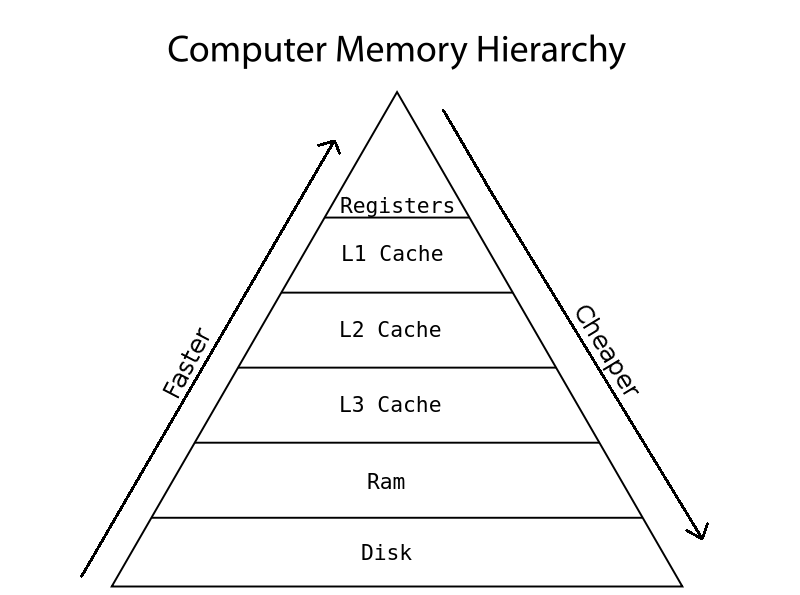
\includegraphics[scale=.54]{./include/pics/memory}
  \caption{Computer Memory Hierarchy}
  \label{fig:mem}
\end{figure}
Another more accurate abstraction is that shown in Figure~\ref{fig:mem}.  In a 
sense, the magic really happens when things get into the CPU registers.  But 
something that's in RAM that you want to operate on, as it's headed to the CPU, 
gets cached into various levels of (comparatively) fast access storage along 
the way.  Understanding this behavior, and writing your code to take advantage 
of it, can have \emph{tremendous} impacts on performance.

\begin{figure}[ht]
  \centering
  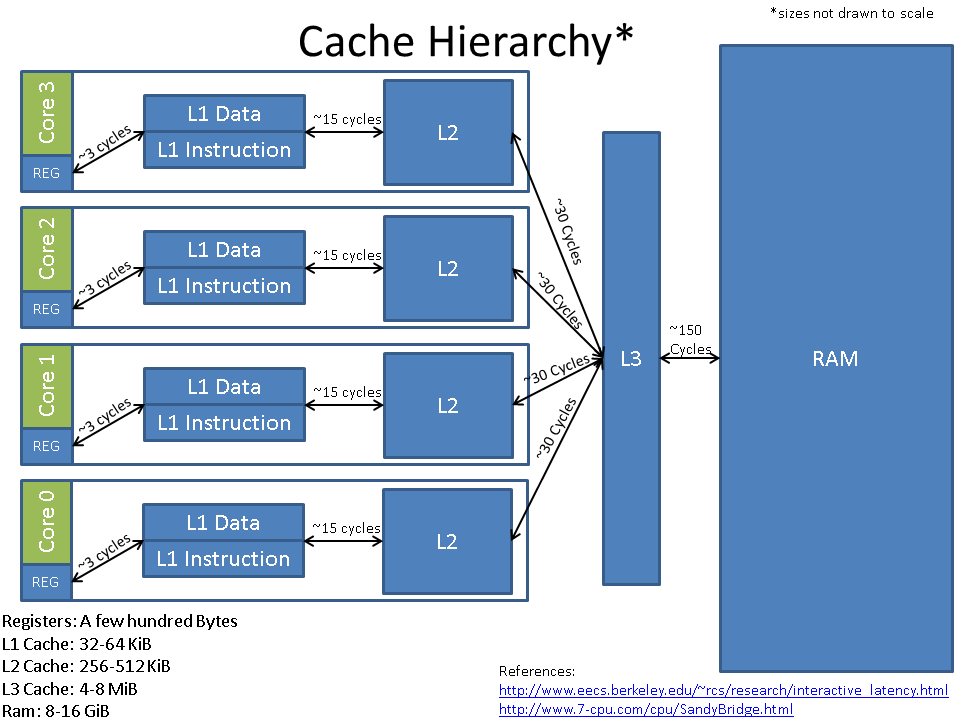
\includegraphics[scale=.54]{./include/pics/cache}
  \caption{Detailed Computer Memory Hierarchy}
  \label{fig:mem2}
\end{figure}
A more detailed presentation of Figure~\ref{fig:mem} is that found in 
Figure~\ref{fig:mem2}.  Here we see a more accurate presentation; for example, 
L3 cache (if it exists) is shared by all cores on a moder CPU, with L2 private, 
and L1 split into data and instruction caches.  The lookup costs in terms of 
processor cycles are provided for each type of memory.  These ``times'' are 
presented in terms of the CPU cycle for mostly historical reasons, though there 
is benefit to thinking in these terms (for example, when trying to minimize 
wait cycles).  Though note that a faster processor could actually 
\emph{increase} these costs, specifically RAM to L3 lookups.

If you are unfamiliar with the importance (or existence) of cache, I would 
strongly encourage you to experiment with this great
\href{http://www.overbyte.com.au/misc/Lesson3/CacheFun.html}%
{interactive visualization} 
showing (relative) speeds of cache misses. It too involves some simplifications 
of how modern hardware actually works, so if this is at all confusing, let us 
all take a moment to pity the tragic life of the computer engineer.  Another 
great resource is this
\href{http://www.eecs.berkeley.edu/~rcs/research/interactive_latency.html}%
{interactive visualization} showing memory and cache latency numbers by year.





\paragraph{Cache Misses} Fundamentally, a cache miss occurs when the cache 
needs some piece of data to pass along to registers, but it isn't immediately 
available and the computer has to go digging through RAM (or god help you, 
disk) to get it.  Cache misses are bad and reduce performance.  You can't get 
rid of them completely, unless your entire problem --- copies and all --- 
comfortably fits into cache, but you can eliminate \emph{unnecessary} cache 
misses being aware of how your data and algorithms interact with cache.  See 
the demo \code{cache_access.r} in \thispackage for an example of good versus 
bad cache access.
